\documentclass[10pt,a4paper]{article}
\usepackage{tikz}
\usetikzlibrary{matrix}
\usetikzlibrary{decorations.markings}

\tikzset{->-/.style={decoration={
            markings,
            mark=at position #1 with {\arrow{>}}},postaction={decorate}}}
\begin{document}
     \begin{figure}[htp]
        \centering
        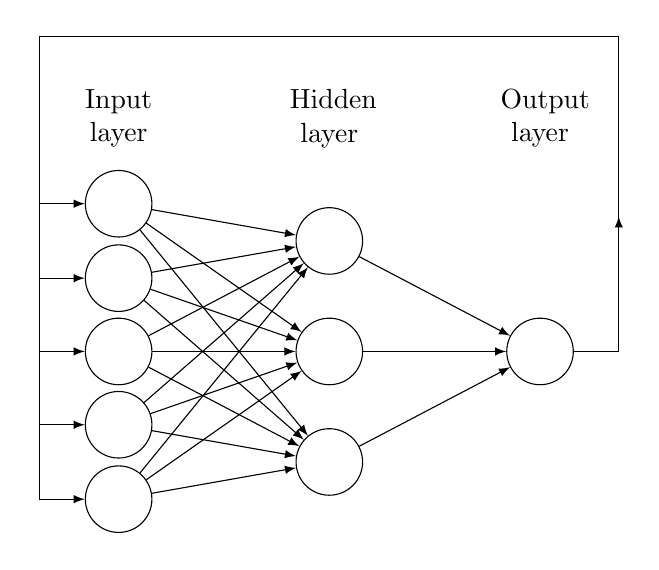
\begin{tikzpicture}[
            plain/.style={
                draw=none,
                fill=none,
            },
            net/.style={
                matrix of nodes,
                nodes={
                    draw,
                    circle,
                    inner sep=8.5pt
                },
                nodes in empty cells,
                column sep=0.6cm,
                row sep=-11pt
            },
            >=latex
            ]
            \matrix[net] (mat)
            {
                |[plain]| \parbox{1cm}{\centering Input\\layer} & |[plain]| \parbox{1cm}{\centering Hidden\\layer} & |[plain]| \parbox{1cm}{\centering Output\\layer} \\
                & |[plain]| \\
                |[plain]| & \\
                & |[plain]| \\
                |[plain]| & |[plain]| \\
                & & \\
                |[plain]| & |[plain]| \\
                & |[plain]| \\
                |[plain]| & \\
                & |[plain]| \\
            };
        \draw[->-=.5] (mat-6-3) --  ++(1cm,0)--++(0,4cm)coordinate(a);
            \foreach \ai [count=\mi ]in {2,4,...,10}
            \draw[<-] (mat-\ai-1) --  ++(-1cm,0)|-(a);
            \foreach \ai in {2,4,...,10}
            {\foreach \aii in {3,6,9}
                \draw[->] (mat-\ai-1) -- (mat-\aii-2);
            }
            \foreach \ai in {3,6,9}
            \draw[->] (mat-\ai-2) -- (mat-6-3);
%           \draw[->] (mat-6-3) --  ++(1cm,0)--++(0,4cm)coordinate(a);
        \end{tikzpicture}
        
        \caption{Multilayer feedforward neural network with one hidden layer.}
        \label{hiddenlayer}
     \end{figure} 
\end{document}